%% Преамбула TeX-файла

% 1. Стиль и язык
\documentclass[utf8x, 12pt]{G7-32} % Стиль (по умолчанию будет 14pt)

% Остальные стандартные настройки убраны в preamble.inc.tex.
\sloppy

% Настройки стиля ГОСТ 7-32
% Для начала определяем, хотим мы или нет, чтобы рисунки и таблицы нумеровались в пределах раздела, или нам нужна сквозная нумерация.
\EqInChapter % формулы будут нумероваться в пределах раздела
\TableInChapter % таблицы будут нумероваться в пределах раздела
\PicInChapter % рисунки будут нумероваться в пределах раздела
\usepackage{slashbox}

% Добавляем гипертекстовое оглавление в PDF
\usepackage[
bookmarks=true, colorlinks=true, unicode=true,
urlcolor=black,linkcolor=black, anchorcolor=black,
citecolor=black, menucolor=black, filecolor=black,
]{hyperref}

% Изменение начертания шрифта --- после чего выглядит таймсоподобно.
% apt-get install scalable-cyrfonts-tex

\IfFileExists{cyrtimes.sty}
    {
        \usepackage{cyrtimespatched}
    }
    {
        % А если Times нету, то будет CM...
    }

\usepackage{graphicx}   % Пакет для включения рисунков

% С такими оно полями оно работает по-умолчанию:
% \RequirePackage[left=20mm,right=10mm,top=20mm,bottom=20mm,headsep=0pt]{geometry}
% Если вас тошнит от поля в 10мм --- увеличивайте до 20-ти, ну и про переплёт не забывайте:
\geometry{right=20mm}
\geometry{left=30mm}


% Пакет Tikz
\usepackage{tikz}
\usetikzlibrary{arrows,positioning,shadows}

% Произвольная нумерация списков.
\usepackage{enumerate}

% ячейки в несколько строчек
\usepackage{multirow}

% itemize внутри tabular
\usepackage{paralist,array}

% Центрирование подписей к плавающим окружениям
\usepackage[justification=centering]{caption}


% Настройки листингов.
\ifPDFTeX
% 8 Листинги

\usepackage{listings}
\usepackage{wrapfig}
% Значения по умолчанию
\lstset{
  basicstyle= \footnotesize,
  breakatwhitespace=true,% разрыв строк только на whitespacce
  breaklines=true,       % переносить длинные строки
%   captionpos=b,          % подписи снизу -- вроде не надо
  inputencoding=koi8-r,
  numbers=left,          % нумерация слева
  numberstyle=\footnotesize,
  showspaces=false,      % показывать пробелы подчеркиваниями -- идиотизм 70-х годов
  showstringspaces=false,
  showtabs=false,        % и табы тоже
  stepnumber=1,
  tabsize=4,              % кому нужны табы по 8 символов?
  frame=single,
  escapeinside={(*}{*)}, %выделение
  literate={а}{{\selectfont\char224}}1
  {б}{{\selectfont\char225}}1
  {в}{{\selectfont\char226}}1
  {г}{{\selectfont\char227}}1
  {д}{{\selectfont\char228}}1
  {е}{{\selectfont\char229}}1
  {ё}{{\"e}}1
  {ж}{{\selectfont\char230}}1
  {з}{{\selectfont\char231}}1
  {и}{{\selectfont\char232}}1
  {й}{{\selectfont\char233}}1
  {к}{{\selectfont\char234}}1
  {л}{{\selectfont\char235}}1
  {м}{{\selectfont\char236}}1
  {н}{{\selectfont\char237}}1
  {о}{{\selectfont\char238}}1
  {п}{{\selectfont\char239}}1
  {р}{{\selectfont\char240}}1
  {с}{{\selectfont\char241}}1
  {т}{{\selectfont\char242}}1
  {у}{{\selectfont\char243}}1
  {ф}{{\selectfont\char244}}1
  {х}{{\selectfont\char245}}1
  {ц}{{\selectfont\char246}}1
  {ч}{{\selectfont\char247}}1
  {ш}{{\selectfont\char248}}1
  {щ}{{\selectfont\char249}}1
  {ъ}{{\selectfont\char250}}1
  {ы}{{\selectfont\char251}}1
  {ь}{{\selectfont\char252}}1
  {э}{{\selectfont\char253}}1
  {ю}{{\selectfont\char254}}1
  {я}{{\selectfont\char255}}1
  {А}{{\selectfont\char192}}1
  {Б}{{\selectfont\char193}}1
  {В}{{\selectfont\char194}}1
  {Г}{{\selectfont\char195}}1
  {Д}{{\selectfont\char196}}1
  {Е}{{\selectfont\char197}}1
  {Ё}{{\"E}}1
  {Ж}{{\selectfont\char198}}1
  {З}{{\selectfont\char199}}1
  {И}{{\selectfont\char200}}1
  {Й}{{\selectfont\char201}}1
  {К}{{\selectfont\char202}}1
  {Л}{{\selectfont\char203}}1
  {М}{{\selectfont\char204}}1
  {Н}{{\selectfont\char205}}1
  {О}{{\selectfont\char206}}1
  {П}{{\selectfont\char207}}1
  {Р}{{\selectfont\char208}}1
  {С}{{\selectfont\char209}}1
  {Т}{{\selectfont\char210}}1
  {У}{{\selectfont\char211}}1
  {Ф}{{\selectfont\char212}}1
  {Х}{{\selectfont\char213}}1
  {Ц}{{\selectfont\char214}}1
  {Ч}{{\selectfont\char215}}1
  {Ш}{{\selectfont\char216}}1
  {Щ}{{\selectfont\char217}}1
  {Ъ}{{\selectfont\char218}}1
  {Ы}{{\selectfont\char219}}1
  {Ь}{{\selectfont\char220}}1
  {Э}{{\selectfont\char221}}1
  {Ю}{{\selectfont\char222}}1
  {Я}{{\selectfont\char223}}1
}

% Стиль для псевдокода: строчки обычно короткие, поэтому размер шрифта побольше
\lstdefinestyle{pseudocode}{
  basicstyle=\small,
  keywordstyle=\color{black}\bfseries\underbar,
  language=Pseudocode,
  numberstyle=\footnotesize,
  commentstyle=\footnotesize\it
}

% Стиль для обычного кода: маленький шрифт
\lstdefinestyle{realcode}{
  basicstyle=\scriptsize,
  numberstyle=\footnotesize
}

% Стиль для коротких кусков обычного кода: средний шрифт
\lstdefinestyle{simplecode}{
  basicstyle=\footnotesize,
  numberstyle=\footnotesize
}

% Стиль для BNF
\lstdefinestyle{grammar}{
  basicstyle=\footnotesize,
  numberstyle=\footnotesize,
  stringstyle=\bfseries\ttfamily,
  language=BNF
}

% Определим свой язык для написания псевдокодов на основе Python
\lstdefinelanguage[]{Pseudocode}[]{Python}{
  morekeywords={each,empty,wait,do},% ключевые слова добавлять сюда
  morecomment=[s]{\{}{\}},% комменты {а-ля Pascal} смотрятся нагляднее
  literate=% а сюда добавлять операторы, которые хотите отображать как мат. символы
    {->}{\ensuremath{$\rightarrow$}~}2%
    {<-}{\ensuremath{$\leftarrow$}~}2%
    {:=}{\ensuremath{$\leftarrow$}~}2%
    {<--}{\ensuremath{$\Longleftarrow$}~}2%
}[keywords,comments]

% Свой язык для задания грамматик в BNF
\lstdefinelanguage[]{BNF}[]{}{
  morekeywords={},
  morecomment=[s]{@}{@},
  morestring=[b]",%
  literate=%
    {->}{\ensuremath{$\rightarrow$}~}2%
    {*}{\ensuremath{$^*$}~}2%
    {+}{\ensuremath{$^+$}~}2%
    {|}{\ensuremath{$|$}~}2%
}[keywords,comments,strings]

% Подписи к листингам на русском языке.
\renewcommand\lstlistingname{\cyr\CYRL\cyri\cyrs\cyrt\cyri\cyrn\cyrg}
\renewcommand\lstlistlistingname{\cyr\CYRL\cyri\cyrs\cyrt\cyri\cyrn\cyrg\cyri}

\else
\usepackage{local-minted}
\fi

% Полезные макросы листингов.
% Любимые команды
\newcommand{\Code}[1]{\textbf{#1}}


\begin{document}

\frontmatter % выключает нумерацию ВСЕГО; здесь начинаются ненумерованные главы: реферат, введение, глоссарий, сокращения и прочее.

% Команды \breakingbeforechapters и \nonbreakingbeforechapters
% управляют разрывом страницы перед главами.
% По-умолчанию страница разрывается.

% \nobreakingbeforechapters
% \breakingbeforechapters

% Также можно использовать \Referat, как в оригинале
%\begin{abstract}
%	Титульный лист. Эта страница нужна мне, чтобы не сбивалась нумерация страниц
%	\cite{Dh}
%	\cite{Bayer}
%	\cite{Habr1}
%	\cite{Noise_func}
%	\cite{Ulich}

%Это пример каркаса расчётно-пояснительной записки, желательный к использованию в РПЗ проекта по курсу РСОИ.

%Данный опус, как и более новые версии этого документа, можно взять по адресу (\url{https://github.com/rominf/latex-g7-32}).

%Текст в документе носит совершенно абстрактный характер.
%\end{abstract}
% НАЧАЛО ТИТУЛЬНОГО ЛИСТА
\begin{center}
	\hfill \break
	\textit{
		\normalsize{Государственное образовательное учреждение высшего профессионального образования}}\\ 
	
	\textit{
		\normalsize  {\bf  «Московский государственный технический университет}\\ 
		\normalsize  {\bf имени Н. Э. Баумана»}\\
		\normalsize  {\bf (МГТУ им. Н.Э. Баумана)}\\
	}
	\noindent\rule{\textwidth}{2pt}
	\hfill \break
	\noindent
	\makebox[0pt][l]{ФАКУЛЬТЕТ}%
	\makebox[\textwidth][c]{«Информатика и системы управления»}%
	\\
	\noindent
	\makebox[0pt][l]{КАФЕДРА}%
	\makebox[\textwidth][r]{«Программное обеспечение ЭВМ и информационные технологии»}%
	\\
	\hfill\break
	\hfill \break
	\hfill \break
	\hfill \break
	\normalsize{\bf Р А С Ч Ё Т Н О - П О Я С Н И Т Е Л Ь Н А Я\space\space З А П И С К А}\\
	\normalsize{\bf к курсовой работе на тему:}\\
	\hfill \break
	\large{Мониторинг вызовов функций ядра Linux}\\
	\hfill \break
	\hfill \break
	\hfill \break
	\hfill \break
	\hfill \break	
	\normalsize {
		\noindent
		\makebox[0pt][l]{Студент}%
		\makebox[\textwidth][c]{}%
		\makebox[0pt][r]{{$\underset{\text{(Подипсь, дата)}}{\underline{\hspace{8cm}}}$ \space Камакин А.С.}}
	}\\
	\hfill \break	
	\normalsize {
		\noindent
		\makebox[0pt][l]{Руководитель курсового проекта}%
		\makebox[\textwidth][c]{ ~~~~~~~~      }%
		\makebox[0pt][r]{{$\underset{\text{(Подпись, дата)}}{\underline{\hspace{6cm}}}$ \space Ковтушенко А.П.}}
	}
	\hfill \break
	\hfill \break
	\hfill \break
	\hfill \break
\end{center}
\hfill \break
\hfill \break
\begin{center} Москва 2018 \end{center}

\thispagestyle{empty} % 
% КОНЕЦ ТИТУЛЬНОГО ЛИСТА


%%% Local Variables: 
%%% mode: latex
%%% TeX-master: "rpz"
%%% End: 

\tableofcontents


%%% Local Variables:
%%% mode: latex
%%% TeX-master: "rpz"
%%% End:

%
%%% Local Variables:
%%% mode: latex
%%% TeX-master: "rpz"
%%% End:


\Introduction

Иногда, при работе с Linux-системами, требуется перехватывать вызовы важных функций внутри ядра (вроде открытия файлов и запуска процессов) для обеспечения возможности мониторинга активности в системе или превентивного блокирования деятельности подозрительных процессов.

Проект посвящен исследованию способов перехвата вызовов функций внутри ядра с их последующей отправкой на удаленный компьютер из пространства ядра. Целью проекта является разработка подхода, позволяющего удобно перехватить любую функцию в ядре по имени и выполнить свой код вокруг её вызовов с последующей отправкой данных на удаленный компьютер.

\mainmatter % это включает нумерацию глав и секций в документе ниже

\chapter{Аналитический раздел}
\label{cha:analysis}
%
% % В начале раздела  можно напомнить его цель
%
В соответствии с заданием на курсовой проект необходимо разработать программное
обеспечение, перехватывающее события в системе, инициирующиеся средством исполнения экспортируемых функций ядра. Так же эту информацию необходимо передавать на удаленный компьютер.
Программное обеспечение должно обеспечивать перехват всех действий нужных функций и обеспечивать пользователю возможность удаленно ее анализировать.


% Обратите внимание, что включается не ../dia/..., а inc/dia/...
% В Makefile есть соответствующее правило для inc/dia/*.pdf, которое
% берет исходные файлы из ../dia в этом случае.



\section{Анализ подходов реализации}

\begin{itemize}
	\item Linux Security API
	\item Модификация таблицы системных вызовов
	\item Использование kprobes
	\item Сплайсинг
	\item Новый подход с ftrace
	\end{itemize}

\subsection{Linux Security API}
Наиболее правильным было бы использование Linux Security API — специального интерфейса, созданного именно для этих целей. В критических местах ядерного кода расположены вызовы security-функций, которые в свою очередь вызывают коллбеки, установленные security-модулем. Security-модуль может изучать контекст операции и принимать решение о её разрешении или запрете.

К сожалению, у Linux Security API есть пара важных ограничений:
\begin{itemize}
	\item security-модули не могут быть загружены динамически, являются частью ядра и требуют его пересборки
	\item в системе может быть только один security-модуль (с небольшими исключениями)
\end{itemize}

Если по поводу множественности модулей позиция разработчиков ядра неоднозначная, то запрет на динамическую загрузку принципиальный: security-модуль должен быть частью ядра, чтобы обеспечивать безопасность постоянно, с момента загрузки. Таким образом, для использования Security API необходимо поставлять собственную сборку ядра, а также интегрировать дополнительный модуль с SELinux или AppArmor, которые используются популярными дистрибутивами.

\subsection{Модификация таблицы системных вызовов}
Мониторинг требовался в основном для действий, выполняемых пользовательскими приложениями, так что в принципе мог бы быть реализован на уровне системных вызовов. Как известно, Linux хранит все обработчики системных вызовов в таблице sys\_call\_table. Подмена значений в этой таблице приводит к смене поведения всей системы. Таким образом, сохранив старое значения обработчика и подставив в таблицу собственный обработчик, мы можем перехватить любой системный вызов.

У этого подхода есть определённые преимущества:
\begin{itemize}
	\item Полный контроль над любыми системными вызовами — единственным интерфейсом к ядру у пользовательских приложений. Используя его мы можем быть уверены, что не пропустим какое-нибудь важное действие, выполняемое пользовательским процессом.
	\item Минимальные накладные расходы. Есть единоразовые капитальные вложения при обновлении таблицы системных вызовов. Помимо неизбежной полезной нагрузки мониторинга, единственным расходом является лишний вызов функции (для вызова оригинального обработчика системного вызова).
	\item Минимальные требования к ядру. При желании этот подход не требует каких-либо дополнительных конфигурационных опций в ядре, так что в теории поддерживает максимально широкий спектр систем.
\end{itemize}

Однако, подход не лишен недостатков:
\begin{itemize}
	\item Техническая сложность реализации. Сама по себе замена указателей в таблице не представляет трудностей. Но сопутствующие задачи требуют неочевидных решений и определённой квалификации:
	\begin{itemize}
		\item поиск таблицы системных вызовов
		\item обход защиты от модификации таблицы
		\item атомарное и безопасное выполнение замены
	\end{itemize}
	\item Невозможность перехвата некоторых обработчиков. В ядрах до версии 4.16 обработка системных вызовов для архитектуры x86\_64 содержала целый ряд оптимизаций. Некоторые из них требовали того, что обработчик системного вызова являлся специальным переходничком, реализованным на ассемблере. Соответственно, подобные обработчики порой сложно, а иногда и вовсе невозможно заменить на свои, написанные на Си. Более того, в разных версиях ядра используются разные оптимизации, что добавляет в копилку технических сложностей.
	\item Перехватываются только системные вызовы. Этот подход позволяет заменять обработчики системных вызовов, что ограничивает точки входа только ими. Все дополнительные проверки выполняются либо в начале, либо в конце, и у нас есть лишь аргументы системного вызова и его возвращаемое значение. Иногда это приводит к необходимости дублировать проверки на адекватность аргументов и проверки доступа. Иногда вызывает лишние накладные расходы, когда требуется дважды копировать память пользовательского процесса: если аргумент передаётся через указатель, то его сначала придётся скопировать нам самим, затем оригинальный обработчик скопирует аргумент ещё раз для себя. Кроме того, в некоторых случаях системные вызовы предоставляют слишком низкую гранулярность событий, которые приходится дополнительно фильтровать от шума.
\end{itemize}

Данный подход позволяет полностью подменить таблицу системных вызовов что является несомненным плюсом, но также ограничивает количество функций, которые можно мониторить.

\subsection{Использование kprobes}
Одним из вариантов, которые рассматривались, было использование kprobes: специализированного API, в первую очередь предназначенного для отладки и трассирования ядра. Этот интерфейс позволяет устанавливать пред- и постобработчики для любой инструкции в ядре, а также обработчики на вход и возврат из функции. Обработчики получают доступ к регистрам и могут их изменять. Таким образом, можно было бы получить как мониторинг, так и возможность влиять на дальнейший ход работы.

Преимущества, которые даёт использование kprobes для перехвата:
\begin{itemize}
	\item Зрелый API. Kprobes существуют и улучшаются с 2002 года. Они обладают хорошо задокументированным интерфейсом, большинство подводных камней уже найдено, их работа по возможности оптимизирована.
	\item Перехват любого места в ядре. Kprobes реализуются с помощью точек останова (инструкции int3), внедряемых в исполнимый код ядра. Это позволяет устанавливать kprobes в буквально любом месте любой функции, если оно известно. Аналогично, kretprobes реализуются через подмену адреса возврата на стеке и позволяют перехватить возврат из любой функции (за исключением тех, которые управление в принципе не возвращают).
\end{itemize}

Недостатки kprobes:

\begin{itemize}
	\item Техническая сложность. Kprobes — это только способ установить точку останова в любом места ядра. Для получения аргументов функции или значений локальных переменных надо знать, в каких регистрах или где на стеке они лежат, и самостоятельно их оттуда извлекать. Для блокировки вызова функции необходимо вручную модифицировать состояние процесса так, чтобы процессор подумал, что он уже вернул управление из функции.
	\item Jprobes объявлены устаревшими. Jprobes — это надстройка над kprobes, позволяющая удобно перехватывать вызовы функций. Она самостоятельно извлечёт аргументы функции из регистров или стека и вызовет ваш обработчик, который должен иметь ту же сигнатуру, что и перехватываемая функция. Подвох в том, что jprobes объявлены устаревшими и вырезаны из современных ядер.
	\item Нетривиальные накладные расходы. Расстановка точек останова дорогая, но она выполняется единоразово. Точки останова не влияют на остальные функции, однако их обработка относительно недешёвая. К счастью, для архитектуры x86\_64 реализована jump-оптимизация, существенно уменьшающая стоимость kprobes, но она всё ещё остаётся больше, чем, например, при модификации таблицы системных вызовов.
	\item Ограничения kretprobes. Kretprobes реализуются через подмену адреса возврата на стеке. Соответственно, им необходимо где-то хранить оригинальный адрес, чтобы вернуться туда после обработки kretprobe. Адреса хранятся в буфере фиксированного размера. В случае его переполнения, когда в системе выполняется слишком много одновременных вызовов перехваченной функции, kretprobes будет пропускать срабатывания.
	\item Отключенное вытеснение. Так как kprobes основывается на прерываниях и жонглирует регистрами процессора, то для синхронизации все обработчики выполняются с отключенным вытеснением (preemption). Это накладывает определённые ограничения на обработчики: в них нельзя ждать — выделять много памяти, заниматься вводом-выводом, спать в таймерах и семафорах, и прочие известные вещи.
\end{itemize}

\subsection{Сплайсинг}
Классический способ перехвата функций, заключающийся в замене инструкций в начале функции на безусловный переход, ведущий в обработчик. Оригинальные инструкции переносятся в другое место и исполняются перед переходом обратно в перехваченную функцию. С помощью двух переходов вшивается (splice in) свой дополнительный код в функцию, поэтому такой подход называется сплайсингом.

Именно таким образом и реализуется jump-оптимизация для kprobes. Используя сплайсинг можно добиться тех же результатов, но без дополнительных расходов на kprobes и с полным контролем ситуации.

Преимущества сплайсинга:
\begin{itemize}
	\item Минимальные требования к ядру. Сплайсинг не требует каких-либо особенных опций в ядре и работает в начале любой функции. Нужно только знать её адрес.
	\item Минимальные накладные расходы. Два безусловных перехода — вот и все действия, которые надо выполнить перехваченному коду, чтобы передать управление обработчику и обратно. Подобные переходы отлично предсказываются процессором и являются очень дешёвыми.
\end{itemize}

Недостатки:
\begin{itemize}
	\item Техническая сложность. Она зашкаливает. Нельзя просто так взять и переписать машинный код. Вот краткий и неполный список задач, которые придётся решить:
	\begin{itemize}
		\item синхронизация установки и снятия перехвата (что если функцию вызовут прямо в процессе замены её инструкций?)
		\item обход защиты на модификацию регионов памяти с кодом
		\item инвалидация кешей процессора после замены инструкций
		\item дизассемблирование заменяемых инструкций, чтобы скопировать их целыми
		\item проверка на отсутствие переходов внутрь заменяемого куска
		\item проверка на возможность переместить заменяемый кусок в другое место
	\end{itemize}
\end{itemize}

\subsection{Новый подход с ftrace}
Ftrace — это фреймворк для трассирования ядра на уровне функций. Он разрабатывается с 2008 года и обладает удобным интерфейсом для пользовательских программ. Ftrace позволяет отслеживать частоту и длительность вызовов функций, отображать графы вызовов, фильтровать интересующие функции по шаблонам, и так далее.

Реализуется ftrace на основе ключей компилятора -pg и -mfentry, которые вставляют в начало каждой функции вызов специальной трассировочной функции mcount() или \_\_fentry\_\_(). Обычно, в пользовательских программах эта возможность компилятора используется профилировщиками, чтобы отслеживать вызовы всех функций. Ядро же использует эти функции для реализации фреймворка ftrace.

Вызывать ftrace из каждой функции — это, разумеется, не дёшево, поэтому для популярных архитектур доступна оптимизация: динамический ftrace. Суть в том, что ядро знает расположение всех вызовов mcount() или \_\_fentry\_\_() и на ранних этапах загрузки заменяет их машинный код на nop — специальную ничего не делающую инструкцию. При включении трассирования в нужные функции вызовы ftrace добавляются обратно. Таким образом, если ftrace не используется, то его влияние на систему минимально.

Преимущества:
\begin{itemize}
	\item Зрелый API и простой код. Использование готовых интерфейсов в ядре существенно упрощает код. Вся установка перехвата требует пары вызовов функций, заполнение двух полей в структуре. Остальной код — это исключительно бизнес-логика, выполняемая вокруг перехваченной функции.
	\item Перехват любой функции по имени. Для указания интересующей нас функции достаточно написать её имя в обычной строке. Не требуются какие-то особые реверансы с редактором связей, разбор внутренних структур данных ядра, сканирование памяти, или что-то подобное. Можно перехватить любую функцию (даже не экспортируемую для модулей), зная лишь её имя.
	\item Перехват совместим с трассировкой. Очевидно, что этот способ не конфликтует с ftrace, так что с ядра всё ещё можно снимать очень полезные показатели производительности. Использование kprobes или сплайсинга может помешать механизмам ftrace.
\end{itemize}

Недостатки:
\begin{itemize}
	\item Требования к конфигурации ядра. Для успешного выполнения перехвата функций с помощью ftrace ядро должно предоставлять целый ряд возможностей:
	\begin{itemize}
		\item список символов kallsyms для поиска функций по имени
		\item фреймворк ftrace в целом для выполнения трассировки
		\item опции ftrace, критически важные для перехвата
	\end{itemize}
\end{itemize}

Все эти возможности не являются критичными для функционирования системы и могут быть отключены в конфигурации ядра. Правда, обычно ядра, используемые популярными дистрибутивами, все эти опции в себе всё равно содержат, так как они не влияют на производительность и полезны при отладке. Однако, если вам необходимо поддерживать какие-то особенные ядра, то следует иметь в виду эти требования.

\begin{itemize}
	\item Накладные расходы на ftrace меньше, чем у kprobes (так как ftrace не использует точки останова), но они выше, чем у сплайсинга, сделанного вручную. Действительно, динамический ftrace, является сплайсингом, только вдобавок выполняющий код ftrace и другие коллбеки.
	\item Оборачиваются функции целиком. Как и традиционный сплайсинг, данный подход полностью оборачивает вызовы функций. Однако, если сплайсинг технически возможно выполнить в любом месте функции, то ftrace срабатывает исключительно при входе. Естественно, обычно это не вызывает сложностей и даже наоборот удобно, но подобное ограничение иногда может быть недостатком.
\end{itemize}

\section{Загружаемые модули ядра Linux }
Ядро Linux относится к категории так называемых монолитных – это означает, что большая часть функциональности операционной системы называется ядром и запускается в привилегированном режиме. Этот подход отличен от подхода микроядра, когда в режиме ядра выполняется только основная функциональность (взаимодействие между процессами [inter-process communication, IPC], диспетчеризация, базовый ввод-вывод [I/O], управление памятью), а остальная функциональность вытесняется за пределы привилегированной зоны (драйверы, сетевой стек, файловые системы). Можно было бы подумать, что ядро Linux очень статично, но на самом деле все как раз наоборот.
Ядро Linux динамически изменяемое – это означает, что вы можете загружать в ядро дополнительную функциональность, выгружать функции из ядра и даже добавлять новые модули, использующие другие модули ядра. Преимущество загружаемых модулей заключается в возможности сократить расход памяти для ядра, загружая только необходимые модули (это может оказаться важным для встроенных систем) \cite{book4}

Linux – не единственное (и не первое) динамически изменяемое монолитное ядро. Загружаемые модули поддерживаются в BSD-системах, Sun Solaris, в ядрах более старых операционных систем, таких как OpenVMS, а также в других популярных ОС, таких как Microsoft Windows и Apple Mac OS X.
\subsection{Устройство модуля ядра}
Загружаемые модули ядра имеют ряд фундаментальных отличий от элементов, интегрированных непосредственно в ядро, а также от обычных программ. Обычная программа содержит главную процедуру (main)в отличие от загружаемого модуля, содержащего функции входа и выхода (в версии 2.6 эти функции можно именовать как угодно). Функция входа вызывается, когда модуль загружается в ядро, а функция выхода – соответственно при выгрузке из ядра. Поскольку функции входа и выхода являются пользовательскими, для указания назначения этих функций используются макросы module\_init и module\_exit . Загружаемый модуль содержит также набор обязательных и дополнительных макросов. Они определяют тип лицензии, автора и описание модуля, а также другие параметры. Пример очень простого загружаемого модуля приведен на рисунке  \ref{fig:an01} .
\begin{figure}[h!]
	\centering
	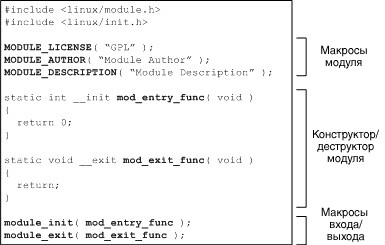
\includegraphics[width=0.6\textwidth]{img/1.png}
	\caption{Пример загружаемого модуля с разделами ELF}
	\label{fig:an01}
\end{figure}
\subsection{Объектный код модуля ядра}
Загружаемый модуль представляет собой просто специальный объектный файл в формате ELF (Executable and Linkable Format). Обычно объектные файлы обрабатываются компоновщиком, который разрешает символы и формирует исполняемый файл. Однако в связи с тем, что загружаемый модуль не может разрешить символы до загрузки в ядро, он остается ELF-объектом. Для работы с загружаемыми модулями можно использовать стандартные средства работы с объектными файлами (которые в версии 2.6 имеют суффикс .ko, от kernel object). Например, если вывести информацию о модуле утилитой objdump, вы обнаружите несколько привычных разделов, в том числе .text (инструкции), .data (инициализированные данные) и .bss (Block Started Symbol или неинициализированные данные)\cite{book4}

В модуле также обнаружатся дополнительные разделы, ответственные за поддержку его динамического поведения. Раздел .init.text содержит код module\_init, а раздел .exit.text – код module\_exit code (рисунок  \ref{fig:an02}). Раздел .modinfo содержит тексты макросов, указывающие тип лицензии, автора, описание и т.д.
\begin{figure}[h!]
	\centering
	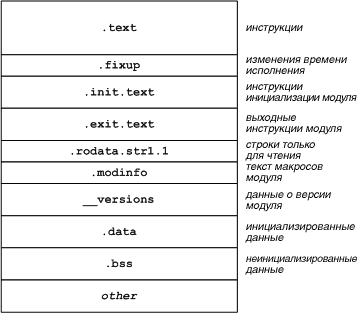
\includegraphics[width=0.6\textwidth]{img/2.png}
	\caption{Пример загружаемого модуля с разделами ELF}
	\label{fig:an02}
\end{figure}
\subsection{Жизненный цикл загружаемого модуля ядра}
Процесс загрузки модуля начинается в пользовательском пространстве с команды insmod (вставить модуль). Команда insmod определяет модуль для загрузки и выполняет системный вызов уровня пользователя init\_module для начала процесса загрузки. Команда insmod для ядра версии 2.6 стала чрезвычайно простой (70 строк кода) за счет переноса части работы в ядро. Команда insmod не выполняет никаких действий по разрешению символов (вместе с командой kerneld), а просто копирует двоичный код модуля в ядро при помощи функции init\_module; остальное делает само ядро.

Функция init\_module работает на уровне системных вызовов и вызывает функцию ядра sys\_init\_module (рисунок  \ref{fig:an03}). Это основная функция для загрузки модуля, обращающаяся к нескольким другим функциям для решения специальных задач. Аналогичным образом команда rmmod выполняет системный вызов функции delete\_module, которая обращается в ядро с вызовом sys\_delete\_module для удаления модуля из ядра.
\begin{figure}[h!]
	\centering
	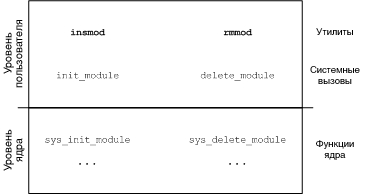
\includegraphics[width=0.6\textwidth]{img/3.png}
	\caption{ Основные команды и функции, участвующие в загрузке и выгрузке модуля}
	\label{fig:an03}
\end{figure}
\subsection{Подробности загрузки модуля}
Теперь давайте взглянем на внутренние функции для загрузки модуля (рисунок \ref{fig:an04}). При вызове функции ядра sys\_init\_module сначала выполняется проверка того, имеет ли вызывающий соответствующие разрешения (при помощи функции capable). Затем вызывается функция load\_module, которая выполняет механическую работу по размещению модуля в ядре и производит необходимые операции (я вскоре расскажу об этом). Функция load\_module возвращает ссылку, которая указывает на только что загруженный модуль. Затем он вносится в двусвязный список всех модулей в системе, и все потоки, ожидающие изменения состояния модуля, уведомляются при помощи специального списка. В конце вызывается функция init() и статус модуля обновляется, чтобы указать, что он загружен и доступен.
\begin{figure}[h!]
	\centering
	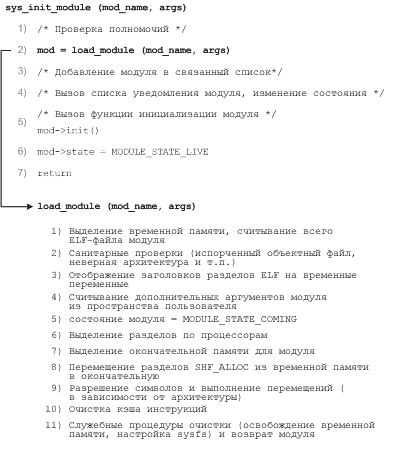
\includegraphics[width=0.6\textwidth]{img/4.png}
	\caption{ Внутренний процесс загрузки модуля(в упрощенном виде)}
	\label{fig:an04}
\end{figure}
Внутренние процессы загрузки модуля представляют собой анализ и управление модулями ELF. Функция load\_module (которая находится в ./linux/kernel/module.c) начинает с выделения блока временной памяти для хранения всего модуля ELF. Затем модуль ELF считывается из пользовательского пространства во временную память при помощи copy\_from\_user. Являясь объектом ELF, этот файл имеет очень специфичную структуру, которая легко поддается анализу и проверке.

Следующим шагом является ряд "санитарных проверок" загруженного образа (является ли ELF-файл допустимым? соответствует ли он текущей архитектуре? и так далее). После того как проверка пройдена, образ ELF анализируется и создается набор вспомогательных переменных для заголовка каждого раздела, чтобы облегчить дальнейший доступ к ним. Поскольку базовый адрес объектного файла ELF равен 0 (до перемещения), эти переменные включают соответствующие смещения в блок временной памяти. Во время создания вспомогательных переменных также проверяются заголовки разделов ELF, чтобы убедиться, что загружаемый модуль корректен.

Дополнительные параметры модуля, если они есть, загружаются из пользовательского пространства в другой выделенный блок памяти ядра (шаг 4), и статус модуля обновляется, чтобы обозначить, что он загружен (MODULE\_STATE\_COMING). Если необходимы данные для процессоров (согласно результатам проверки заголовков разделов), для них выделяется отдельный блок.

В предыдущих шагах разделы модуля загружались в память ядра (временную), и было известно, какие из них используются постоянно, а какие могут быть удалены. На следующем шаге (7) для модуля в памяти выделяется окончательное расположение, и в него перемещаются необходимые разделы (обозначенные в заголовках SHF\_ALLOC или расположенные в памяти во время выполнения). Затем производится дополнительное выделение памяти размера, необходимого для требуемых разделов модуля. Производится проход по всем разделам во временном блоке ELF,, и те из них, которые необходимы для выполнения, копируются в новый блок. Затем следуют некоторые служебные процедуры. Также происходит разрешение символов, как расположенных в ядре (включенных в образ ядра при компиляции), так и временных (экспортированных из других модулей).

Затем производится проход по оставшимся разделам и выполняются перемещения. Этот шаг зависит от архитектуры и соответственно основывается на вспомогательных функциях, определенных для данной архитектуры (./linux/arch/<arch>/kernel/module.c). В конце очищается кэш инструкций (поскольку использовались временные разделы .text), выполняется еще несколько служебных процедур (очистка памяти временного модуля, настройка sysfs) и, в итоге, модуль возвращает load\_module
\subsection{Подробности выгрузки модуля}

Выгрузка модуля фактически представляет собой зеркальное отражение процесса загрузки за исключением того, что для безопасного удаления модуля необходимо выполнить несколько "санитарных проверок". Выгрузка модуля начинается в пользовательском пространстве с выполнения команды rmmod (удалить модуль). Внутри команды rmmod выполняется системный вызов delete\_module, который в конечном счете инициирует sys\_delete\_module внутри ядра (см рисунок \ref{fig:an03} ). Основные операции удаления модуля показаны на рисунке  \ref{fig:an05}.
\begin{figure}[h!]
	\centering
	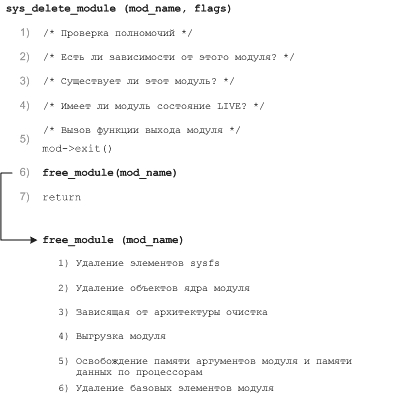
\includegraphics[width=0.6\textwidth]{img/5.png}
	\caption{  Внутренний процесс выгрузки модуля(в упрощенном виде)}
	\label{fig:an05}
\end{figure}
При вызове функции ядра sys\_delete\_module (с именем удаляемого модуля в качестве параметра) сначала выполняется проверка того, имеет ли вызывающий соответствующие разрешения. Затем по списку проверяются зависимости других модулей от данного модуля. При этом используется список modules\_which\_use\_me, содержащий по элементу для каждого зависимого модуля. Если список пуст, т.е. зависимостей не обнаружено, то модуль становится кандидатом на удаление (иначе возвращается ошибка). Затем проверяется, загружен ли модуль. Ничто не запрещает пользователю запустить команду rmmod для модуля, который в данный момент устанавливается, поэтому данная процедура проверяет, активен ли модуль. После нескольких дополнительных служебных проверок предпоследним шагом вызывается функция выхода данного модуля (предоставляемая самим модулем). В заключение вызывается функция free\_module.

К моменту вызова free\_module уже известно, что модуль может быть безопасно удален. Зависимостей не обнаружено, и для данного модуля можно начать процесс очистки ядра. Этот процесс начинается с удаления модуля из различных списков, в которые он был помещен во время установки (sysfs, список модулей и т.д.). Потом инициируется команда очистки, зависящая от архитектуры (она расположена в ./linux/arch/<arch>/kernel/module.c). Затем обрабатываются зависимые модули, и данный модуль удаляется из их списков. В конце, когда с точки зрения ядра очистка завершена, освобождаются различные области памяти, выделенные для модуля, в том числе память для параметров, память для данных по процессорам и память модуля ELF (core и init).

\section{Вывод}
Проанализировав все изученные подходы к реализации мониторинга за вызовами функций ядра, был выбран подход с ftrace. Изначально наиболее подходящим вариантом была подмена таблицу системных вызовов, но при реализации возникли некоторые проблемы:
\begin{itemize}
	\item после релиза ядра версии 3.0, таблицу больше нельзя получить простым импортом нужного модуля, доступ к ней осуществляется посредством поиска по памяти
	\item не работает на ядрах выше версии 4.16, так как участок памяти, в котором она находится, заблокирован, а его разблокировка ведет к ошибке установки модуля
	\item не позволяет следить за чем-то кроме функций, находящихся в таблице системных вызовов.
\end{itemize}
На момент написания программы, использовалось ядро 4.19.12, поэтому лучше всего подходил вариант с ftrace. Подход поддерживает ядра версий 3.19+ для архитектуры x86\_64.

%%% Local Variables:
%%% mode: latex
%%% TeX-master: "rpz"
%%% End:

\chapter{Конструкторский раздел}
\label{cha:design}

\section{Общая архитектура приложения}
В состав программного обеспечения входит только загружаемый модуль ядра, следящий за вызовом нужных функций, с поледующией отправкой информации о них клиенту напрямую из пространства ядра.

\section{Перехват функций}

Каждую перехватываемую функцию можно описать следующей структурой:
\begin{lstlisting}[language=c++,,escapeinside={(@}{@)},caption={ftrace\_hook}]
/**
* struct ftrace_hook - описывает перехватываемую функцию
*
* @name:       имя перехватываемой функции
*
* @function:   адрес функции-обёртки, которая будет вызываться вместо
*              перехваченной функции
*
* @original:   указатель на место, куда следует записать адрес
*              перехватываемой функции, заполняется при установке
*
* @address:    адрес перехватываемой функции, выясняется при установке
*
* @ops:        служебная информация ftrace, инициализируется нулями,
*              при установке перехвата будет доинициализирована
*/
struct ftrace_hook {
	const char *name;
	void *function;
	void *original;

	unsigned long address;
	struct ftrace_ops ops;
};
\end{lstlisting}

Пользователю необходимо заполнить только первые три поля: name, function, original. Остальные поля считаются деталью реализации. Описание всех перехватываемых функций можно собрать в массив и использовать макросы, чтобы повысить компактность кода:

\newpage
\begin{lstlisting}[language=c++,,escapeinside={(@}{@)},caption={ftrace\_hook define}]
#define HOOK(_name, _function, _original)       \
		{                                       \
			.name = (_name),                    \
			.function = (_function),            \
			.original = (_original),            \
		}

static struct ftrace_hook hooked_functions[] = {
	HOOK("sys_clone",   fh_sys_clone,   &real_sys_clone),
};
\end{lstlisting}

Сигнатуры функций должны совпадать один к одному. Без этого, очевидно, аргументы будут переданы неправильно и всё пойдёт под откос. Для перехвата системных вызовов это важно в меньшей степени, так как их обработчики очень стабильные и для эффективности аргументы принимают в том же порядке, что и сами системные вызовы.

\subsection{Инициализация ftrace}
Для начала нам потребуется найти и сохранить адрес функции, которую мы будем перехватывать. Ftrace позволяет трассировать функции по имени, но нам всё равно надо знать адрес оригинальной функции, чтобы вызывать её.

Добыть адрес можно с помощью kallsyms — списка всех символов в ядре. В этот список входят все символы, не только экспортируемые для модулей. Получение адреса перехватываемой функции выглядит примерно так:
\begin{lstlisting}[language=c++,,escapeinside={(@}{@)},caption={resolve\_hook\_address}]
static int resolve_hook_address(struct ftrace_hook *hook)
{
	hook->address = kallsyms_lookup_name(hook->name);

	if (!hook->address) {
		pr_debug("unresolved symbol: %s\n", hook->name);
		return -ENOENT;
	}

	*((unsigned long*) hook->original) = hook->address;

	return 0;
}
\end{lstlisting}

Дальше необходимо инициализировать структуру ftrace\_ops. В ней обязательным полем является лишь func, указывающая на коллбек, но нам также необходимо установить некоторые важные флаги:
\begin{lstlisting}[language=c++,,escapeinside={(@}{@)},caption={fh\_install\_hook}]
int fh_install_hook(struct ftrace_hook *hook)
{
	int err;
	
	err = resolve_hook_address(hook);
	if (err)
		return err;
	
	hook->ops.func = fh_ftrace_thunk;
	hook->ops.flags = FTRACE_OPS_FL_SAVE_REGS | FTRACE_OPS_FL_IPMODIFY;
	
	err = ftrace_set_filter_ip(&hook->ops, hook->address, 0, 0);
	if (err) {
		pr_debug("ftrace_set_filter_ip() failed: %d\n", err);
		return err;
	}
	
	err = register_ftrace_function(&hook->ops);
	if (err) {
		pr_debug("register_ftrace_function() failed: %d\n", err);
		ftrace_set_filter_ip(&hook->ops, hook->address, 1, 0);
		return err;
	}
	
	return 0;
}
\end{lstlisting}

\newpage
Выключается перехват аналогично, только в обратном порядке:
\begin{lstlisting}[language=c++,,escapeinside={(@}{@)},caption={fh\_remove\_hook}]
void fh_remove_hook(struct ftrace_hook *hook)
{
	int err;
	
	err = unregister_ftrace_function(&hook->ops);
	if (err) {
		pr_debug("unregister_ftrace_function() failed: %d\n", err);
	}
	
	err = ftrace_set_filter_ip(&hook->ops, hook->address, 1, 0);
	if (err) {
		pr_debug("ftrace_set_filter_ip() failed: %d\n", err);
	}
}
\end{lstlisting}

После завершения вызова unregister\_ftrace\_function() гарантируется отсутствие активаций установленного коллбека в системе (а вместе с ним — и наших обёрток). Поэтому мы можем, например, спокойно выгрузить модуль-перехватчик, не опасаясь, что где-то в системе ещё выполняются наши функции.

\subsection{Выполнение перехвата функций}

Ftrace позволяет изменять состояние регистров после выхода из коллбека. Изменяя регистр \%rip — указатель на следующую исполняемую инструкцию,— мы изменяем инструкции, которые исполняет процессор — то есть можем заставить его выполнить безусловный переход из текущей функции в нашу. Таким образом мы перехватываем управление на себя.

Коллбек для ftrace выглядит следующим образом:
\begin{lstlisting}[language=c++,,escapeinside={(@}{@)},caption={fh\_remove\_hook}]
static void notrace fh_ftrace_thunk(unsigned long ip, 
	unsigned long parent_ip, struct ftrace_ops *ops, 
	struct pt_regs *regs)
{
	struct ftrace_hook *hook = container_of(ops, struct ftrace_hook, ops);
	regs->ip = (unsigned long) hook->function;
}
\end{lstlisting}

Функция-обёртка, которая вызывается позже, будет выполняться в том же контексте, что и оригинальная функция. Поэтому там можно делать то же, что позволено делать в перехватываемой функции. Например, если перехватывается обработчик прерывания, то спать в обёртке нельзя.

\subsection{Схема работы перехвата}

Рассмотрим пример: терминале набирается команда ls, чтобы увидеть список файлов в текущей директории. Командный интерпретатор для запуска нового процесса использует пару функций fork() + execve() из стандартной библиотеки языка Си. Внутри эти функции реализуются через системные вызовы clone() и execve() соответственно. Допустим, мы перехватываем системный вызов execve(), чтобы контролировать запуск новых процессов.

В графическом виде перехват функции-обработчика выглядит так:
\begin{figure}[h!]
	\centering
	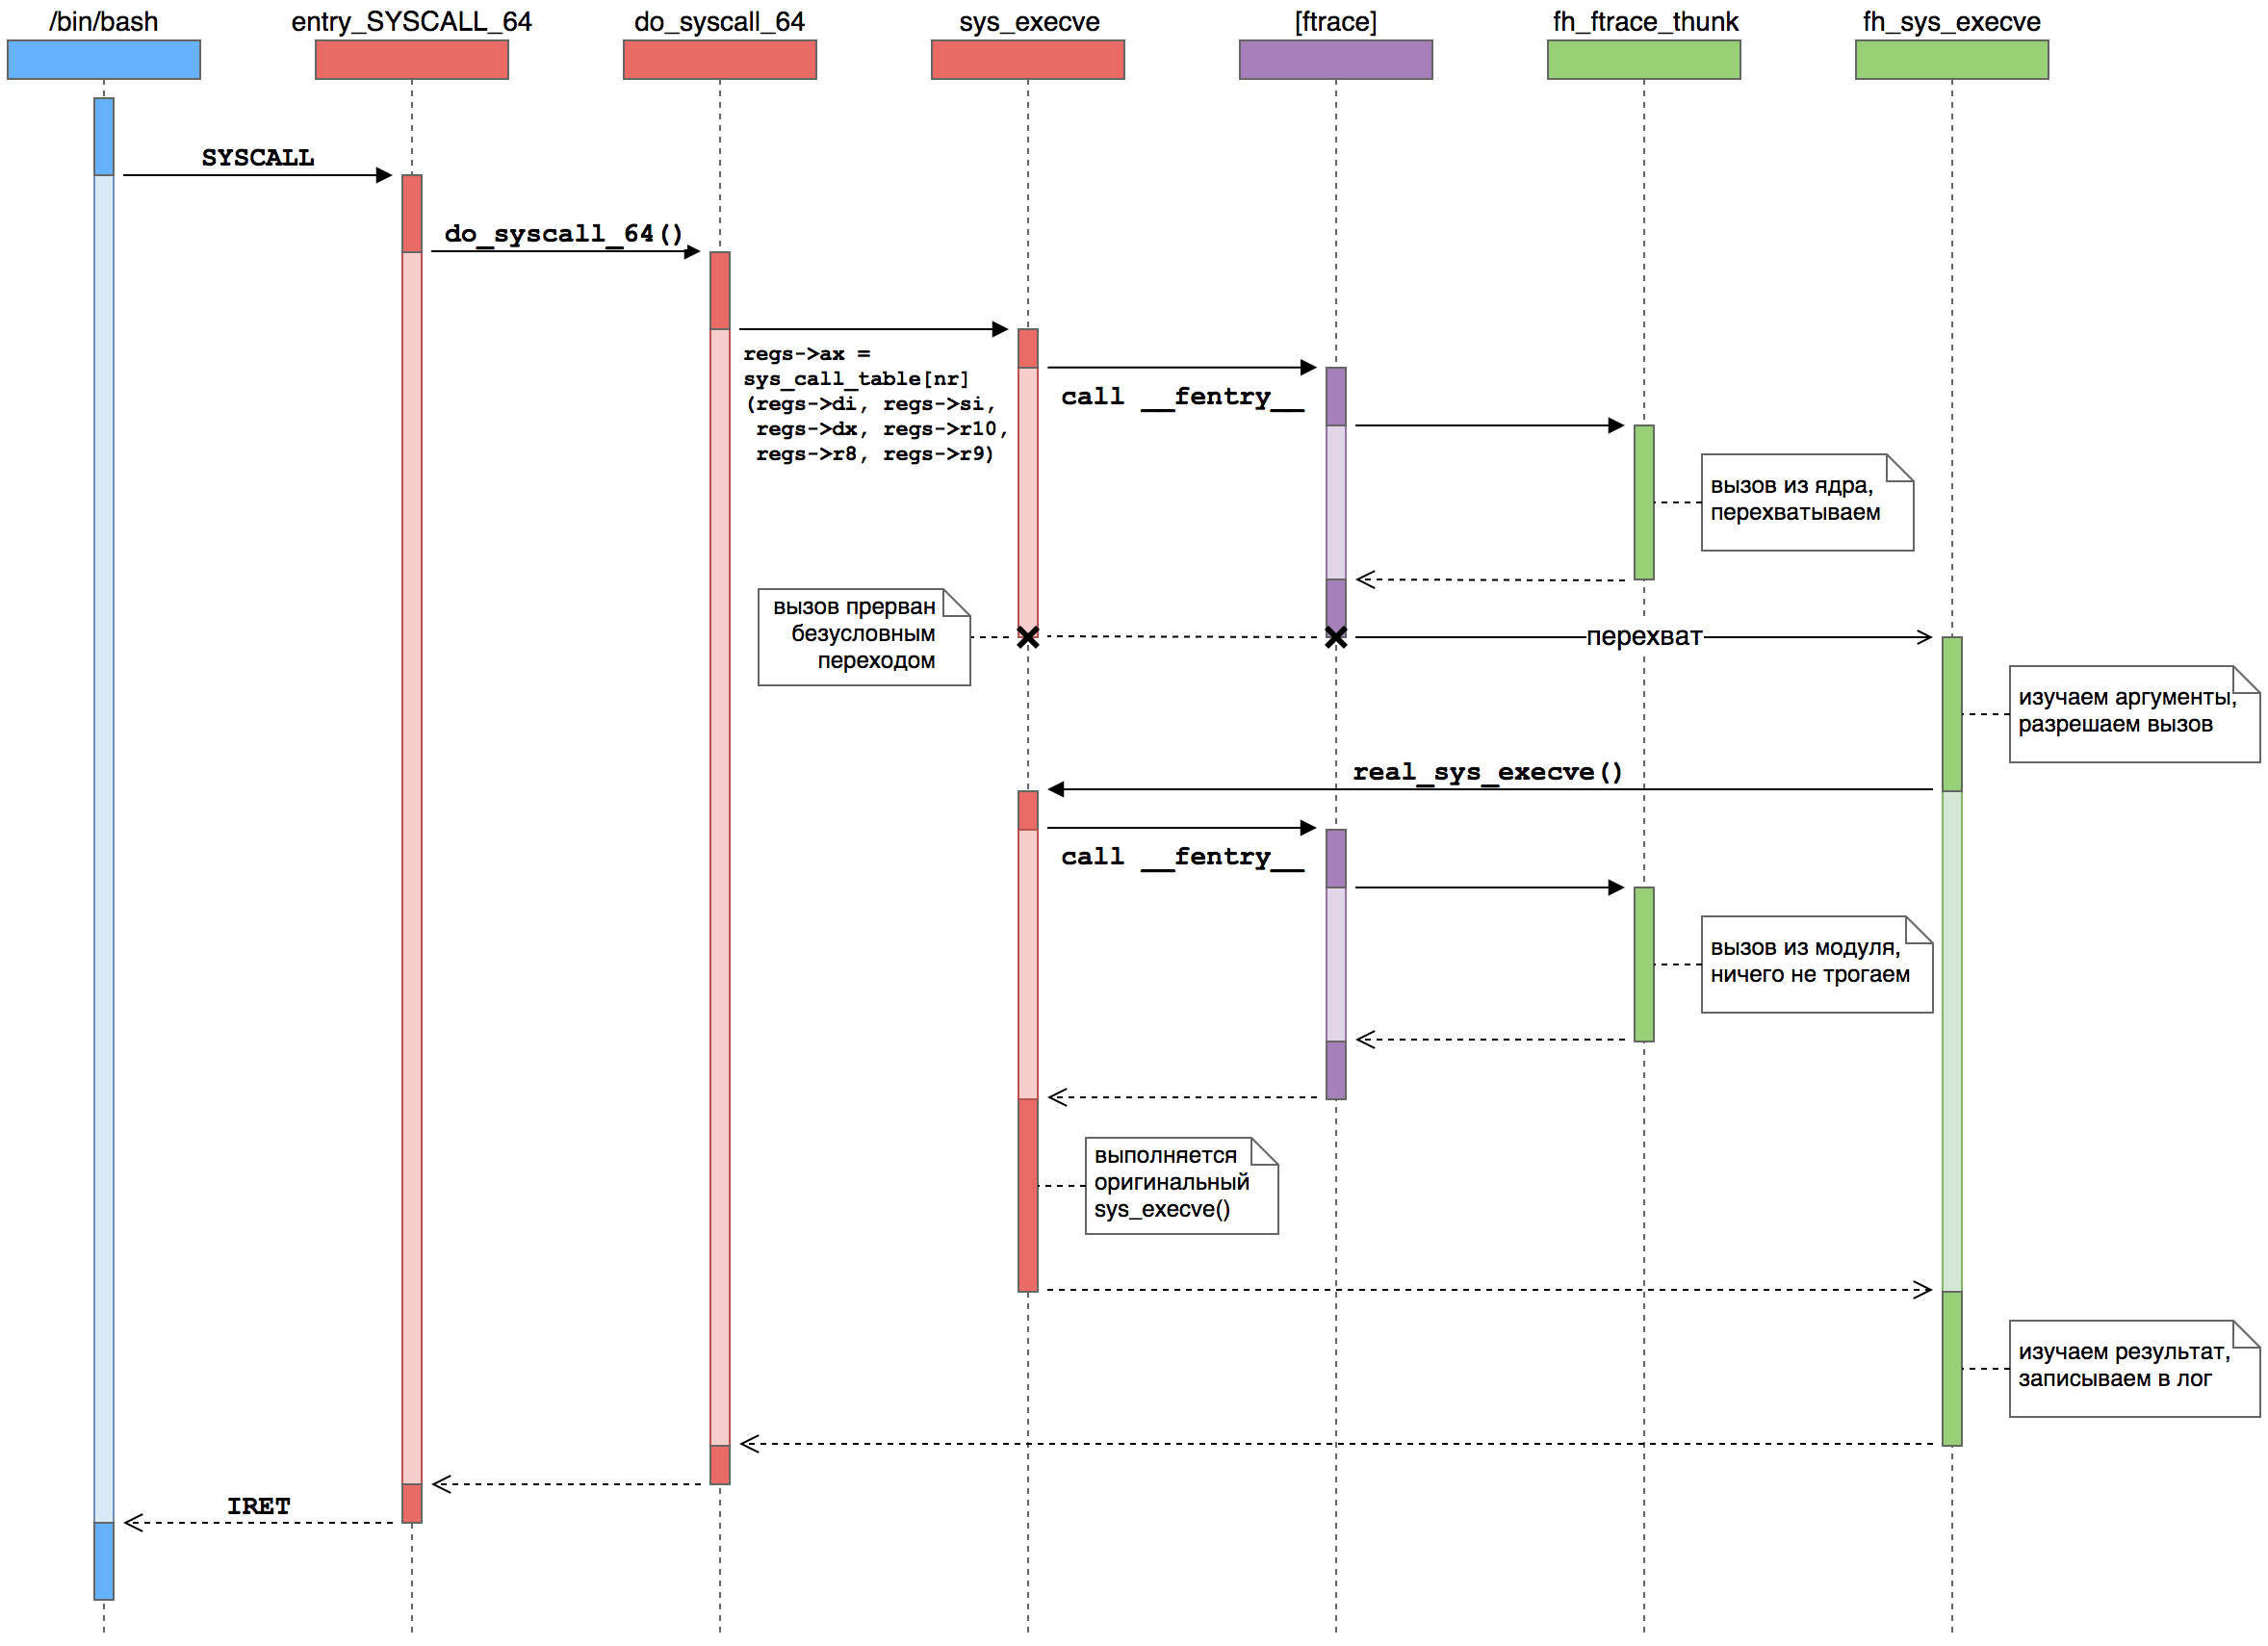
\includegraphics[width=1.0\textwidth]{img/hook_work_scheme.png}
	\caption{Алгоритм работы функции-перехватчика}
	\label{fig:spire00}
\end{figure}

\section{Сервер}


%%% Local Variables:

%%% mode: latex
%%% TeX-master: "rpz"
%%% End:
%--количество цветов
%||количество пикселей
\chapter{Технологический раздел}
\section{Выбор  языка программирования}
Для реализации загружаемого модуля был выбран язык С. 
Операционная система Linux позволяет писать загружаемые модули ядра на Rust и на C. 
Rust непопулярен и ещё только развивается и не обладает достаточным количеством документации.
Для реализации клиента был выбран протокол telnet.
\begin{enumerate}
	 \item Имеется в любой современной ОС. 
	 \item Простота использования.
	 \item Скорость и эффективность.
\end{enumerate}




%%% Local Variables:
%%% mode: latex
%%% TeX-master: "rpz"
%%% End:

%\chapter{Исследовательский раздел}
%\chapter{Заключение}
%\label{cha:research}
%\section{Время дизеринга раличных алгоритмов}

%В данном разделе проводятся вычислительные эксперименты.

%%% Local Variables:
%%% mode: latex
%%% TeX-master: "rpz"
%%% End:

%\chapter{Организационно-экономический раздел}
%\label{cha:econom}
%%% Local Variables:
%%% mode: latex
%%% TeX-master: "rpz"
%%% End:

%\chapter{Промышленная экология и %езопасность}\label{cha:bzd}


%%% Local Variables:
%%% mode: latex
%%% TeX-master: "rpz"
%%% End:


\backmatter %% Здесь заканчивается нумерованная часть документа и начинаются ссылки и
            %% заключение

\Conclusion % заключение к отчёту

В данной работе был реализован загружаемый модуль ядра операционной системы Linux, В процессе разработки нам удалось реализовать подход, позволяющий удобно перехватить любую функцию в ядре по имени и выполнить свой код вокруг её вызовов и сразу отправить нужную информацию клиенту без перехода в режим пользователя. Перехватчик можно устанавливать из загружаемого GPL-модуля, без пересборки ядра. Подход поддерживает ядра версий 3.19+ для архитектуры x86\_64.

%%% Local Variables: 
%%% mode: latex
%%% TeX-master: "rpz"
%%% End: 


% % Список литературы при помощи BibTeX
% Юзать так:
%
% pdflatex rpz
% bibtex rpz
% pdflatex rpz

\bibliographystyle{gost780u}

\begin{thebibliography}{9}
	\bibitem{ftrace} 
	Перехват функций в ядре Linux с помощью ftrace
	\\\texttt{https://m.habr.com/post/413241/}
	
	\bibitem{haifa}
	Haifa Linux Club - Networking Lectures
	\\\texttt{http://haifux.org/network.html}
	
	\bibitem{syscall}
	Loadable Kernel Module Programming and System Call Interception
	\\\texttt{https://www.linuxjournal.com/article/4378}
	
	\bibitem{anatomy} 
	М. Джонс 
	\textit{Анатомия загружаемых модулей ядра Linux}.
	\\\texttt{https://www.ibm.com/developerworks/ru/library/l-lkm/index.html}
	
	\bibitem{sources} 
	Исходные коды ядра Linux
	\\\texttt{http://elixir.free-electrons.com}
\end{thebibliography}


%%% Local Variables: 
%%% mode: latex
%%% TeX-master: "rpz"
%%% End: 


\appendix   % Тут идут приложения

%\chapter{Рисунки, поясняющие работу некоторых функций}
%\label{cha:appendix1}

%\begin{figure}
%\centering
%\caption{Картинка в приложении. Страшная и ужасная.}
%\end{figure}
%\begin{figure}[h!]
%	\centering
%	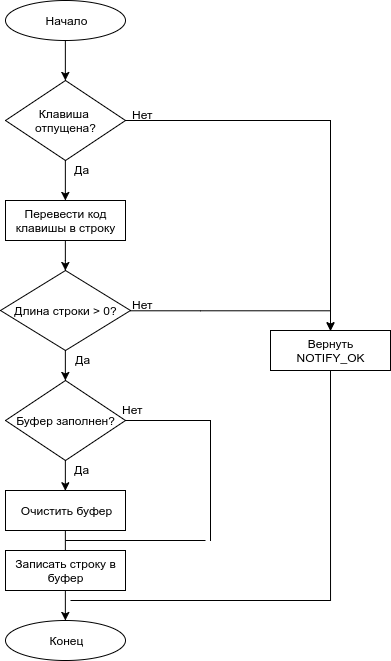
\includegraphics[width=0.6\textwidth]{img/diagram3.png}
%	\caption{Алгоритм работы init-функции}
%	\label{fig:spire02}
%\end{figure}
%\begin{figure}[h!]
%	\centering
%	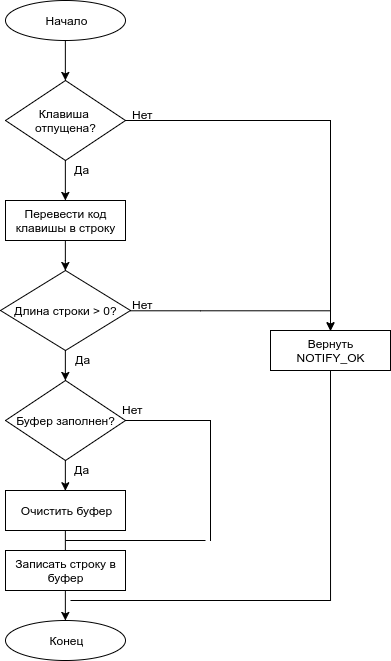
\includegraphics[width=0.6\textwidth]{img/diagram3.png}
%	\caption{Алгоритм работы функции-обработчика}
%	\label{fig:spire03}
%\end{figure}
%%% Local Variables: 
%%% mode: latex
%%% TeX-master: "rpz"
%%% End: 


%%% Local Variables: 
%%% mode: latex
%%% TeX-master: "rpz"
%%% End: 


\end{document}

%%% Local Variables:
%%% mode: latex
%%% TeX-master: t
%%% End:
